% !TEX root = ../../main.tex
\chapter{Resource Allocation}
In this chapter we are going to provide, thanks to a Gantt chart, a general overview of how resources (in this case the two members of the team) have been assigned to various tasks of the project. For the same reasons explained in chapter 3, we provide the assignment of resources also to development, testing and deployment activities.

\begin{figure}[H]
	\begin{adjustwidth}{-2in}{-2in}
		\centering
		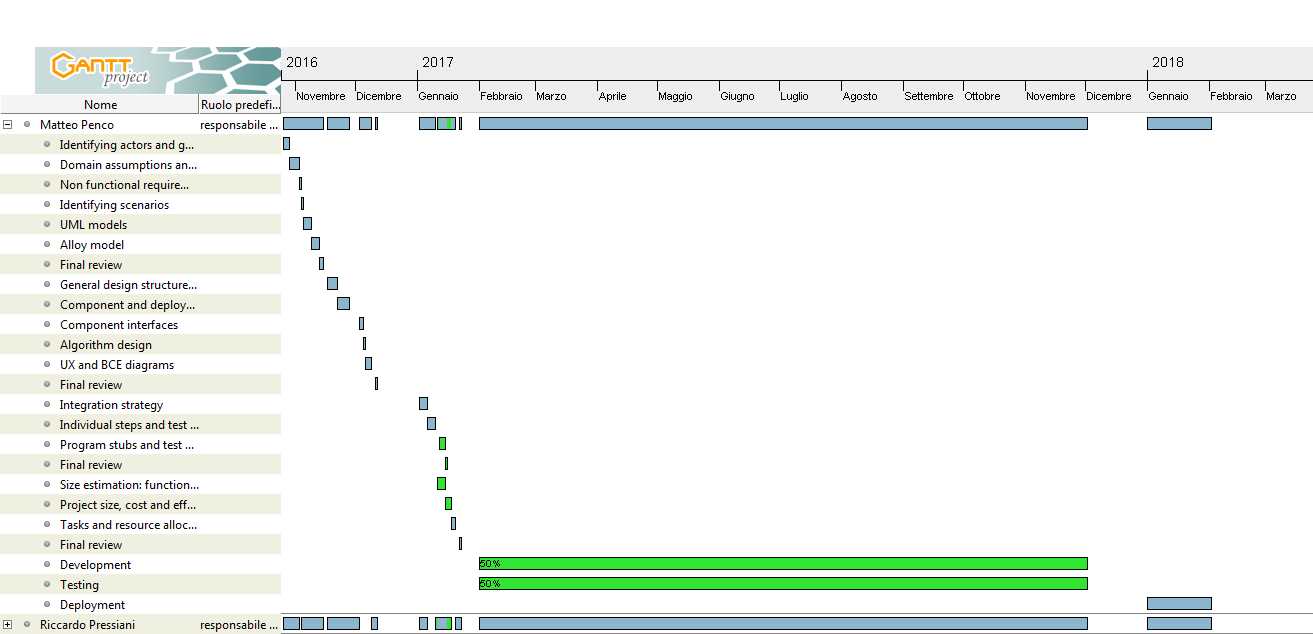
\includegraphics[width=1.5\textwidth]{Resources1}
	\end{adjustwidth}
	\caption[Resource Allocation - Matteo Penco]{The picture above shows the first section of Gantt chart representing resources assigned to various taks of the project.}
	\label{fig:Resources-1}
\end{figure}

\begin{figure}[H]
	\begin{adjustwidth}{-2in}{-2in}
		\centering
		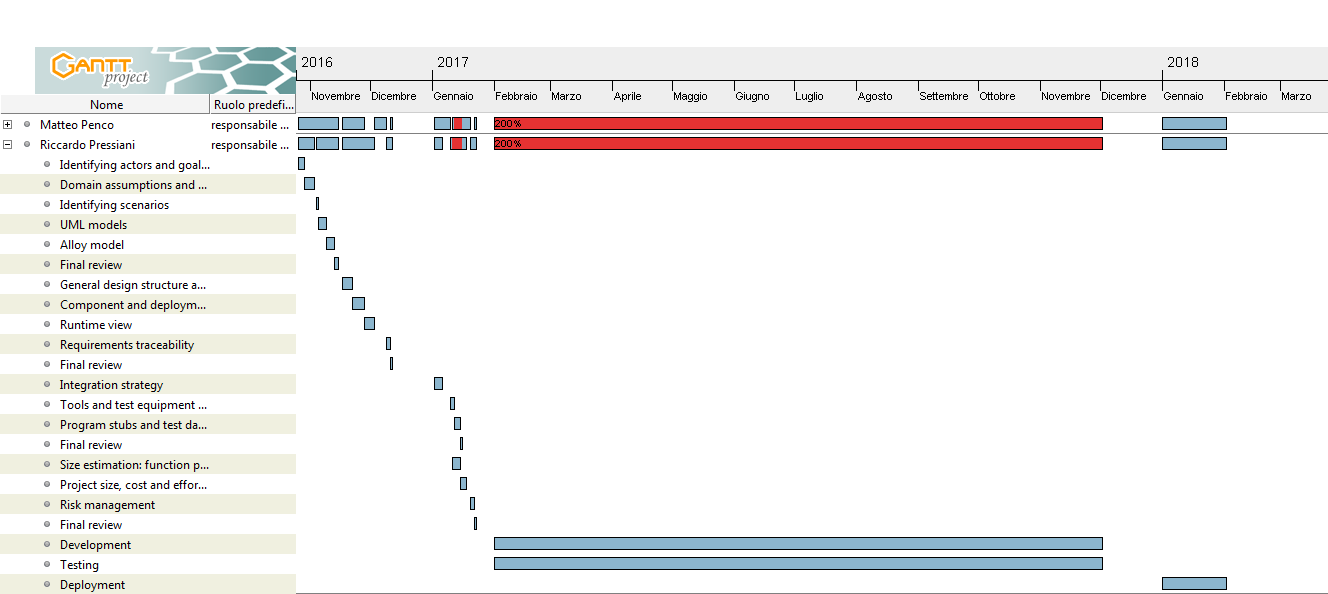
\includegraphics[width=1.5\textwidth]{Resources2}
	\end{adjustwidth}
	\caption[Resources Allocation - Riccardo Pressiani]{The picture above shows the second section of Gantt chart representing resources assigned to various taks of the project.}
	\label{fig:Resources-2}
\end{figure}